\documentclass{standalone}

\usepackage[OT1]{fontenc}
\renewcommand*\familydefault{\sfdefault}
\usepackage{helvet,sfmath}
\usepackage{siunitx}

\usepackage{tikz}
\usetikzlibrary{arrows,calc,patterns}
% \usetikzlibrary{intersections, calc, arrows.meta}
\usepackage{tikz,tkz-euclide}

\definecolor{Liquid1}{RGB}{157, 110, 144}
\definecolor{Liquid2}{RGB}{232, 211, 230}
\definecolor{Note}{RGB}{54, 40, 76}
\definecolor{Rotate}{RGB}{107, 46, 61} 


\begin{document}

\tikzset{every picture/.style={line width=0.75pt}} %set default line width to 0.75pt        

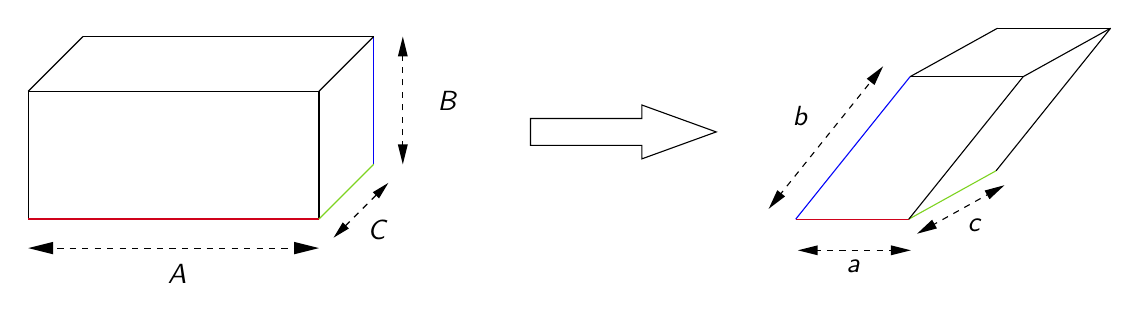
\begin{tikzpicture}[x=0.75pt,y=0.75pt,yscale=-1,xscale=1]
%uncomment if require: \path (0,300); %set diagram left start at 0, and has height of 300

%Straight Lines [id:da41210057881037376] 
\draw    (89,111.45) -- (89,173) ;
%Straight Lines [id:da14965093068588964] 
\draw [color={rgb, 255:red, 4; green, 5; blue, 249 }  ,draw opacity=1 ]   (255.47,85.07) -- (255.47,146.62) ;
%Straight Lines [id:da5219049828348801] 
\draw    (229.09,111.45) -- (229.09,173) ;
%Straight Lines [id:da25069358508747985] 
\draw    (115.38,85.07) -- (255.47,85.07) ;
%Straight Lines [id:da16513842294078795] 
\draw    (89,111.45) -- (229.09,111.45) ;
%Straight Lines [id:da6648386217646297] 
\draw [color={rgb, 255:red, 208; green, 2; blue, 27 }  ,draw opacity=1 ]   (89,173) -- (229.09,173) ;
%Straight Lines [id:da9806882023298378] 
\draw    (89,111.45) -- (115.38,85.07) ;
%Straight Lines [id:da1652703669230915] 
\draw    (229.09,111.45) -- (255.47,85.07) ;
%Straight Lines [id:da7214819227791128] 
\draw [color={rgb, 255:red, 126; green, 211; blue, 33 }  ,draw opacity=1 ]   (229.09,173) -- (255.47,146.62) ;
%Straight Lines [id:da9273538643435697] 
\draw  [dash pattern={on 2.25pt off 2.25pt on 2.25pt off 2.25pt}]  (91,187) -- (227.09,187) ;
\draw [shift={(229.09,187)}, rotate = 180] [fill={rgb, 255:red, 0; green, 0; blue, 0 }  ][line width=0.08]  [draw opacity=0] (12,-3) -- (0,0) -- (12,3) -- cycle    ;
\draw [shift={(89,187)}, rotate = 0] [fill={rgb, 255:red, 0; green, 0; blue, 0 }  ][line width=0.08]  [draw opacity=0] (12,-3) -- (0,0) -- (12,3) -- cycle    ;
%Straight Lines [id:da4363597205858868] 
\draw  [dash pattern={on 2.25pt off 2.25pt on 2.25pt off 2.25pt}]  (237.5,180.59) -- (261.05,157.03) ;
\draw [shift={(262.47,155.62)}, rotate = 135] [fill={rgb, 255:red, 0; green, 0; blue, 0 }  ][line width=0.08]  [draw opacity=0] (8.4,-2.1) -- (0,0) -- (8.4,2.1) -- cycle    ;
\draw [shift={(236.09,182)}, rotate = 315] [fill={rgb, 255:red, 0; green, 0; blue, 0 }  ][line width=0.08]  [draw opacity=0] (8.4,-2.1) -- (0,0) -- (8.4,2.1) -- cycle    ;
%Straight Lines [id:da3286588069139269] 
\draw  [dash pattern={on 2.25pt off 2.25pt on 2.25pt off 2.25pt}]  (269.47,144.62) -- (269.47,87.07) ;
\draw [shift={(269.47,85.07)}, rotate = 90] [fill={rgb, 255:red, 0; green, 0; blue, 0 }  ][line width=0.08]  [draw opacity=0] (9.6,-2.4) -- (0,0) -- (9.6,2.4) -- cycle    ;
\draw [shift={(269.47,146.62)}, rotate = 270] [fill={rgb, 255:red, 0; green, 0; blue, 0 }  ][line width=0.08]  [draw opacity=0] (9.6,-2.4) -- (0,0) -- (9.6,2.4) -- cycle    ;
%Right Arrow [id:dp8675083866086373] 
\draw   (331,124.55) -- (384.68,124.55) -- (384.68,118.07) -- (420.47,131.03) -- (384.68,144) -- (384.68,137.52) -- (331,137.52) -- cycle ;
%Straight Lines [id:da7892767804138988] 
\draw [color={rgb, 255:red, 208; green, 2; blue, 27 }  ,draw opacity=1 ]   (458.76,173.07) -- (513.25,173.07) ;
%Straight Lines [id:da4540617013207512] 
\draw  [dash pattern={on 2.25pt off 2.25pt on 2.25pt off 2.25pt}]  (461.76,188.07) -- (512.25,188.07) ;
\draw [shift={(514.25,188.07)}, rotate = 180] [fill={rgb, 255:red, 0; green, 0; blue, 0 }  ][line width=0.08]  [draw opacity=0] (9.6,-2.4) -- (0,0) -- (9.6,2.4) -- cycle    ;
\draw [shift={(459.76,188.07)}, rotate = 0] [fill={rgb, 255:red, 0; green, 0; blue, 0 }  ][line width=0.08]  [draw opacity=0] (9.6,-2.4) -- (0,0) -- (9.6,2.4) -- cycle    ;
%Straight Lines [id:da09919494460467349] 
\draw [color={rgb, 255:red, 126; green, 211; blue, 33 }  ,draw opacity=1 ]   (513.25,173.07) -- (555.35,149.71) ;
%Straight Lines [id:da1406640131435345] 
\draw  [dash pattern={on 2.25pt off 2.25pt on 2.25pt off 2.25pt}]  (519,179.1) -- (557.6,157.68) ;
\draw [shift={(559.35,156.71)}, rotate = 150.98] [fill={rgb, 255:red, 0; green, 0; blue, 0 }  ][line width=0.08]  [draw opacity=0] (9.6,-2.4) -- (0,0) -- (9.6,2.4) -- cycle    ;
\draw [shift={(517.25,180.07)}, rotate = 330.98] [fill={rgb, 255:red, 0; green, 0; blue, 0 }  ][line width=0.08]  [draw opacity=0] (9.6,-2.4) -- (0,0) -- (9.6,2.4) -- cycle    ;
%Straight Lines [id:da8766628712218499] 
\draw [color={rgb, 255:red, 4; green, 5; blue, 249 }  ,draw opacity=1 ]   (513.87,104.42) -- (458.76,173.07) ;
%Straight Lines [id:da8596487623190532] 
\draw  [dash pattern={on 2.25pt off 2.25pt on 2.25pt off 2.25pt}]  (447.01,166.51) -- (499.62,100.98) ;
\draw [shift={(500.87,99.42)}, rotate = 128.76] [fill={rgb, 255:red, 0; green, 0; blue, 0 }  ][line width=0.08]  [draw opacity=0] (9.6,-2.4) -- (0,0) -- (9.6,2.4) -- cycle    ;
\draw [shift={(445.76,168.07)}, rotate = 308.76] [fill={rgb, 255:red, 0; green, 0; blue, 0 }  ][line width=0.08]  [draw opacity=0] (9.6,-2.4) -- (0,0) -- (9.6,2.4) -- cycle    ;
%Straight Lines [id:da9279338747454127] 
\draw    (513.87,104.42) -- (555.98,81.07) ;
%Straight Lines [id:da24818543539001758] 
\draw    (513.87,104.42) -- (568.36,104.42) ;
%Straight Lines [id:da7272343611427398] 
\draw    (513.25,173.07) -- (568.36,104.42) ;
%Straight Lines [id:da14236804238147438] 
\draw    (568.36,104.42) -- (610.47,81.07) ;
%Straight Lines [id:da07053729233816874] 
\draw    (555.98,81.07) -- (610.47,81.07) ;
%Straight Lines [id:da5325546449751062] 
\draw    (610.47,81.07) -- (555.35,149.71) ;

% Text Node
\draw (155,193.4) node [anchor=north west][inner sep=0.75pt]    {$A$};
% Text Node
\draw (251.28,172.21) node [anchor=north west][inner sep=0.75pt]    {$C$};
% Text Node
\draw (285,110.4) node [anchor=north west][inner sep=0.75pt]    {$B$};
% Text Node
\draw (482,191.47) node [anchor=north west][inner sep=0.75pt]    {$a$};
% Text Node
\draw (540.3,171.79) node [anchor=north west][inner sep=0.75pt]    {$c$};
% Text Node
\draw (456,117.4) node [anchor=north west][inner sep=0.75pt]    {$b$};


\end{tikzpicture}

\end{document}